\section{AI Layer}
\label{sec:ai}

\subsection{Overview}
\label{sec:ai-overview}

The AI layer sits on top of the Knowledge Graph and provides both the user and
the system with access to an AI model that has structured context about what is
happening on the machine. It is not a chatbot grafted onto an existing OS; it
is an interface that can query the graph, invoke application capabilities
through a standardized protocol, and optionally act autonomously when the user
explicitly enables that.

The AI layer is not the primary reason this system exists. The desktop, the
permission system, the profile isolation, and the store all stand on their own.
AI is an enhancement that becomes more useful as the Knowledge Graph fills in
over time, and users who want none of it can disable it completely without
losing any other functionality.

Three principles govern the design of this layer.

\paragraph{Query-first.}
The AI responds when asked. Nothing happens in the background without an
explicit trigger. Autonomous features exist but are separate opt-ins, not
defaults that the user has to find and disable.

\paragraph{Provider-agnostic.}
The system does not care whether the model runs locally or in the cloud.
Every provider implements the same interface; the rest of the codebase never
speaks to a specific backend. The user decides what runs where, including
routing sensitive requests to a local model only.

\paragraph{Opt-out at any point.}
The entire layer can be disabled in Settings under AI. When disabled, no local
model runs, no graph queries originate from the AI layer, Waypointer falls back
to standard search, and no MCP servers are active. The setting is not hidden
five menus deep.

\subsection{Cold-Start Behavior}
\label{sec:ai-coldstart}

The Knowledge Graph is empty on a fresh install. An AI feature that promises
contextual awareness but has nothing in the graph yet is worse than no feature
at all: it creates an expectation and immediately fails to meet it. The system
handles this with straightforward communication rather than by faking
usefulness.

During onboarding, AI features are presented with an honest explanation of
what to expect: the assistant learns context gradually as the system is used,
starts with nothing, and becomes more useful over days and weeks. There are no
demo interactions, no placeholder context, and no fabricated examples of what
it will eventually be able to do.

At onboarding the user can optionally seed the graph with existing data from
their current system: browser history, calendar events, and documents. This is
presented as a trade-off, not a recommendation. Each source can be imported
independently, so someone who is comfortable sharing their calendar but not
their browsing history can import only the former. Importing gives the AI
immediately useful context without a multi-week waiting period.

The AI assistant does not surface proactively until a threshold is met: seven
days of usage or a completed manual import. Before that threshold the feature
is accessible but does not advertise itself. The non-AI parts of the system are
functional and complete from the first boot, so there is no gap in usefulness
during this period.

\subsection{Provider Abstraction}
\label{sec:ai-providers}

Different AI providers have different APIs, different latency profiles, and
significantly different privacy implications. Sending the contents of a private
file to a cloud API is appropriate in some contexts and completely unacceptable
in others. The system needs to handle both without the rest of the codebase
caring which provider is active.

The solution is a Rust trait that every AI backend implements. The AI layer
constructs a \texttt{CompletionRequest}, passes it to whichever provider is
configured, and receives a \texttt{CompletionResponse}. No provider-specific
code is visible outside the provider module. The \texttt{\#[async\_trait]}
macro~\cite{async-trait} is a Rust community crate that enables async methods
in traits, which the stable Rust compiler does not yet support natively; it
desugars the async methods into an equivalent form that compiles correctly.

\begin{lstlisting}[language=Rust, caption={AI provider trait}]
#[async_trait]
pub trait AiProvider: Send + Sync {
    async fn complete(
        &self,
        request: CompletionRequest,
    ) -> Result<CompletionResponse>;
    async fn available(&self) -> bool;
    fn name(&self) -> &str;
}
\end{lstlisting}

Figure~\ref{fig:providers} shows how the AI layer relates to the available
backends.

\begin{figure}[htbp]
\centering
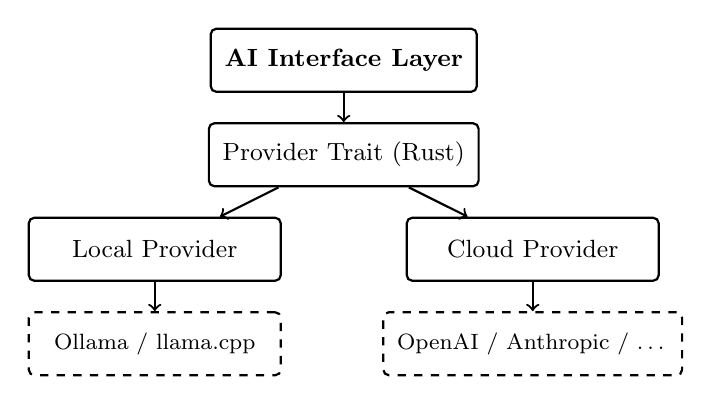
\begin{tikzpicture}[
  box/.style={
    draw, thick, rectangle, rounded corners=2pt,
    minimum width=3.2cm, minimum height=0.8cm,
    font=\small, align=center, inner sep=5pt
  },
  arr/.style={->, thick},
]

\node[box] (ail)   at (0, 3.2) {\textbf{AI Interface Layer}};
\node[box] (trait) at (0, 2.0) {Provider Trait (Rust)};
\node[box] (local) at (-2.4, 0.8) {Local Provider};
\node[box] (cloud) at ( 2.4, 0.8) {Cloud Provider};
\node[box, dashed] (lm)  at (-2.4, -0.4) {\footnotesize Ollama / llama.cpp};
\node[box, dashed] (api) at ( 2.4, -0.4) {\footnotesize OpenAI / Anthropic / \ldots};

\draw[arr] (ail)   -- (trait);
\draw[arr] (trait) -- (local);
\draw[arr] (trait) -- (cloud);
\draw[arr] (local) -- (lm);
\draw[arr] (cloud) -- (api);

\end{tikzpicture}
\caption{Provider abstraction. The AI layer speaks only to the trait; the
concrete backend is a configuration choice. Local and cloud providers are
interchangeable from the perspective of anything above the trait boundary.}
\label{fig:providers}
\end{figure}

\paragraph{Local providers.}
A local provider runs an AI model entirely on the user's machine. No data
leaves the device. The two primary options are \emph{Ollama}~\cite{ollama}
and \emph{llama.cpp}~\cite{llamacpp}.

\emph{llama.cpp} is a C++ inference engine for running large language models
on consumer hardware, originally developed by Georgi Gerganov in 2023. It
achieves viability on consumer hardware through \emph{quantization}: a
technique that reduces the numerical precision of a model's weight values
(for example from 32-bit floats to 4-bit integers), shrinking both the memory
footprint and computation cost at a modest quality trade-off~\cite{llamacpp:quant}.
A 7-billion parameter model that would require roughly 28~GB of RAM at full
32-bit precision runs in approximately 4~GB after 4-bit quantization, which
falls within the RAM budget of a typical consumer laptop. llama.cpp exposes
an HTTP API compatible with the OpenAI request format, so any client written
for the OpenAI API works against a local llama.cpp instance by changing the
base URL.

\emph{Ollama} wraps llama.cpp and other backends in a higher-level tool that
adds model management (download, version tracking, storage), a simpler CLI,
and a REST API. For most users, Ollama is the practical entry point. llama.cpp
is available as a direct option for cases where fine-grained control over
quantization levels and inference parameters is needed.

Both are supported as local provider backends. The specific model is a user
configuration choice. As of 2025, models in the 7B--13B parameter range with
4-bit quantization offer the best balance of quality, memory footprint, and
inference speed on consumer hardware without a dedicated GPU.

\paragraph{Cloud providers.}
Cloud providers send the request to a remote API over HTTPS and return the
response. The system ships with built-in support for the
OpenAI~\cite{openai:api} and Anthropic~\cite{anthropic:api} APIs, both of
which follow similar request/response formats. Additional providers can be
added by implementing the provider trait; the interface is intentionally
minimal. API keys are stored in the system keyring (not in a config file) and
are never written to the Knowledge Graph.

\paragraph{Routing policy.}
Multiple providers can be active simultaneously under a routing policy the
user configures in TOML. The baseline: use the local provider if one is
configured and available; fall back to cloud if the local model is unavailable
or if the request exceeds the local model's context window. Additional rules
can be layered on top: route all code-related requests to a specific provider;
prevent any request that includes personal file contents or graph data from
leaving the machine; route requests originating from a specific application to
a designated provider. Rules are evaluated in order; the first match wins.

\subsection{MCP Integration}
\label{sec:mcp}

\emph{MCP} (Model Context Protocol) is an open protocol published by Anthropic
in November 2024 that standardizes how AI models interact with external tools
and data sources~\cite{mcp:spec}. The core idea is a client/server split: the
AI model talks to an \emph{MCP client}, which in turn dispatches to one or more
\emph{MCP servers}. Each server exposes a list of \emph{tools} (functions the
AI can call) and \emph{resources} (data the AI can read). The protocol runs
over JSON-RPC~2.0~\cite{jsonrpc2}, a lightweight remote procedure call format,
typically over a Unix socket or stdio pipe for local servers and over HTTP/SSE
for remote ones.

The key property of MCP is that the AI model does not need to know anything
about the application it is talking to. A model that has never seen this OS
can still call \texttt{list\_directory} on the file manager MCP server,
because the tool definition (name, parameters, description) is discovered at
runtime. This makes MCP servers independently deployable and the AI layer
application-agnostic.

In this system, first-party applications expose MCP servers as part of their
standard implementation via the \emph{os-sdk} boilerplate described in
Section~\ref{sec:overview}: the file manager exposes \texttt{list\_directory},
\texttt{open\_file}, and \texttt{move\_file}; the terminal exposes
\texttt{run\_command} and \texttt{get\_output}; the Knowledge Graph exposes a
query interface. The AI can coordinate across multiple applications in a single
interaction by calling their respective servers in sequence.
Figure~\ref{fig:mcp} shows the topology.

\begin{figure}[htbp]
	\centering
	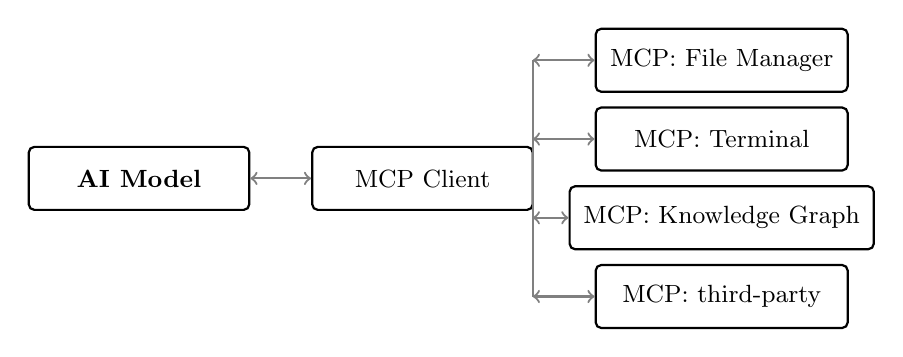
\begin{tikzpicture}[
		box/.style={
			draw, thick, rectangle, rounded corners=2pt,
			minimum width=2.8cm, minimum height=0.8cm,
			font=\small, align=center, inner sep=5pt
		},
		srv/.style={
			draw, thick, rectangle, rounded corners=2pt,
			minimum width=3.2cm, minimum height=0.8cm,
			font=\small, align=center, inner sep=5pt
		},
		arr/.style={<->, thick, gray},
		]
		
		\node[box] (model)  at (0, 0) {\textbf{AI Model}};
		\node[box] (client) at (3.6, 0) {MCP Client};
		
		\node[srv] (fm)   at (7.4,  1.5) {MCP: File Manager};
		\node[srv] (term) at (7.4,  0.5) {MCP: Terminal};
		\node[srv] (kg)   at (7.4, -0.5) {MCP: Knowledge Graph};
		\node[srv] (ext)  at (7.4, -1.5) {MCP: third-party};
		
		\coordinate (mid) at (5.0, 0);
		
		\draw[arr] (model) -- (client);
		\draw[thick, gray] (client.east) -- (mid);
		\draw[thick, gray] (mid |- fm.west)  -- (mid |- ext.west);
		\draw[arr] (mid |- fm.west)   -- (fm.west);
		\draw[arr] (mid |- term.west) -- (term.west);
		\draw[arr] (mid |- kg.west)   -- (kg.west);
		\draw[arr] (mid |- ext.west)  -- (ext.west);
		
	\end{tikzpicture}

\caption{MCP topology. The AI model communicates through a single MCP client
that dispatches to individual application servers. Third-party applications
from the Store can ship their own MCP servers, subject to the permission model
described in Section~\ref{sec:mcp-permissions}.}
\label{fig:mcp}
\end{figure}

CLI tools do not need MCP servers. If a tool has a \texttt{-{}-help} flag and
produces sensible output, the AI can invoke it as a subprocess and read
\texttt{stdout}. MCP is reserved for GUI applications and stateful interfaces
where a subprocess call is insufficient.

\subsection{Interaction Model}
\label{sec:ai-interaction}

\paragraph{Query-based (default).}
The user asks a question, the AI responds. No background activity occurs
without an explicit trigger. The AI has access to the Knowledge Graph and
whatever MCP servers are permitted under the current configuration. Typical
interactions include querying session history, finding files related to a
project, correlating system events with observed behaviour, and composing
multi-step actions across applications.

When a question is asked, the AI layer translates the natural language input
into a Cypher query, executes it against the Knowledge Graph via the Graph
Daemon, and passes the structured results to the model as context. Relative
time expressions are resolved to absolute UTC timestamps before the generation
step, so the model always operates on concrete values rather than ambiguous
phrases. The Cypher generation and the result formatting are two separate model
calls, since combining them causes the model to bias the query toward a
desired-sounding answer rather than accurately querying the schema.

The query validator sits between generation and execution: it checks that the
generated Cypher uses only known node types and relations, contains no write
operations, and includes a \texttt{LIMIT} clause. If validation fails, the
error is fed back for a retry; after two failed attempts the user is told the
question could not be answered, with no silent fallback.

\paragraph{Autonomous agent (explicit opt-in).}
A background agent that observes the event stream and acts proactively is
available as an opt-in capability. It is not enabled by default and each
autonomous behaviour is a separate toggle: suggesting related files when a
document is opened is independent of automatically tagging new files by
project. The agent uses the same provider abstraction and MCP layer as the
query interface; the difference is that it initiates actions rather than
responding to them.

\subsection{Project Context}
\label{sec:ai-project-context}

When a project is active in Focus Mode (Section~\ref{sec:focus-mode}), the AI
layer adjusts its behavior to match. This happens automatically when Focus Mode
activates and is reversed when it deactivates; no separate AI configuration is
required.

\paragraph{Context seed.}
The \texttt{.project} file (Section~\ref{sec:projects}) is loaded as a
structured context seed at the start of every AI query while a project is
focused. The model receives the project name, description, tags, linked
accounts, relevant links, and a summary of recent project activity from the
graph before processing the user's question. This is the minimum context
needed for the AI to give useful answers without the user having to re-explain
their situation every time.

\paragraph{Graph scope.}
If the project's \texttt{[ai]} block declares
\texttt{context\_scope = "project"}, the Graph Daemon restricts the AI
daemon's traversal to nodes carrying a \texttt{PART\_OF} edge to the active
project. The AI sees a narrower but more relevant slice of the graph: recent
project files, sessions where the project was active, applications used in
those sessions, and notifications received during focused work. Nodes outside
the project are not visible to the model for the duration of the focused
session.

This is Access Level~2 from the table in Section~\ref{sec:ai-security}, applied
automatically by Focus Mode rather than requiring the user to configure it
manually per session.

\paragraph{Waypointer integration.}
Inside Waypointer's AI mode (Tab), queries are answered with project context
active. Asking ``which files did I touch yesterday?'' returns results filtered
to the project rather than the full graph. Project-specific quick actions ---
recent files, last commit message, open issues link, focus time this week ---
are derived from live graph queries against the active \texttt{Project} node
and its edges, not from cached or hardcoded data.

\subsection{MCP Permission Model}
\label{sec:mcp-permissions}

MCP servers are the interface through which the AI acts on applications.
The permission model distinguishes between reading information, which the AI
can do by default within the user's configured AI permission level, and
modifying state, which requires explicit per-session authorization.

\begin{table}[htbp]
\caption{Read-only MCP servers (permitted by default)}
\label{tab:mcp-read}
\begin{tabularx}{\linewidth}{lX}
\toprule
\textbf{Server} & \textbf{Exposes} \\
\midrule
File Manager   & Directory listings, file metadata \\
Calendar       & Upcoming and past events \\
Browser        & History and open tabs (no passwords, no form data) \\
System Monitor & Process list and resource usage \\
Notes          & Note titles and content \\
\bottomrule
\end{tabularx}
\end{table}

Reading to answer a question is what the user expects when they ask the AI
something. Answering ``what meetings do I have today?'' without a confirmation
dialog is the correct behaviour. Reading does not change state, and the AI
permission level configured in Settings still gates what data each server
exposes regardless of this default.

\begin{table}[htbp]
\caption{Write and action MCP servers (per-session authorization required)}
\label{tab:mcp-write}
\begin{tabularx}{\linewidth}{lX}
\toprule
\textbf{Server} & \textbf{Can do} \\
\midrule
Terminal     & Execute shell commands \\
File Manager & Create, move, rename, delete files \\
Calendar     & Create and modify events \\
Email        & Compose and send messages \\
Store        & Install and remove packages \\
\bottomrule
\end{tabularx}
\end{table}

Authorization is granted once per session and covers the scope the user
specifies: approving file management does not imply approval for email. It
expires at session end and is not persisted. Within an authorized scope, a
separate hardcoded list of actions always requires explicit confirmation
regardless of session permissions, because their consequences are irreversible
or high-impact: permanent file deletion, sending any external message,
installing or removing system packages, modifying system configuration outside
\texttt{\textasciitilde/.config}, any network request to a host outside the
application's declared permissions, and running commands with elevated
privileges. This list is not configurable.

Third-party MCP servers shipped by Store applications are always treated as
action-requiring by default. A community server that claims to be read-only
receives the same treatment until it carries a verified security audit covering
its MCP implementation.

\subsection{System Explanation Mode}
\label{sec:ai-explain}

A running operating system is largely opaque to its user. Background processes
run, network connections open and close, disk activity spikes, and the user
has no practical way to understand what is happening without opening a terminal
and running several diagnostic commands. This is a gap this system is
positioned to close, because it already has the data.

The AI daemon can answer the question \emph{``What is my computer doing right
now?''} by querying the live event stream and the Knowledge Graph simultaneously.
The event stream provides the current moment: which processes are active, what
they are reading or writing, which network connections are open, what the CPU
and memory usage is and which process owns it. The Knowledge Graph provides
context: whether this activity is normal for this time of day on this machine,
which project the files being accessed belong to, whether this process has
behaved unusually in the past.

The result is a dynamically generated plain-language summary, not a set of
predefined status strings. A typical response might note that the package
manager is fetching updates in the background, that a first-party application
is indexing a recently imported folder, and that network activity is within the
normal range for this time of day. If something is unusual, the summary says
so: a process accessing node types it has never previously accessed, or a
network connection to a destination outside the application's declared
permissions, is flagged in the same natural language response rather than
silently logged.

The explanation mode is available on demand via the AI query interface and as
a persistent ambient view in System Monitor. It does not run continuously in
the background; it is a query like any other, executed when the user asks.
Everything it uses is local: the event stream and the Knowledge Graph never
leave the machine, and the model generating the summary runs locally unless
the user has configured a cloud provider. The output can be shared by the user
if they choose, but nothing is reported automatically.
